\documentclass[17pt]{extarticle}
\usepackage{amsmath}
\usepackage{tikz}
\usepackage[top=0.2in,left=0.9in]{geometry} %This geometry is page layout


\begin{document}
\begin{flushleft}
Geometry Shapes :
\end{flushleft}


\newcommand{\bluecircle}{
    \draw[blue] circle (2);
    }
    


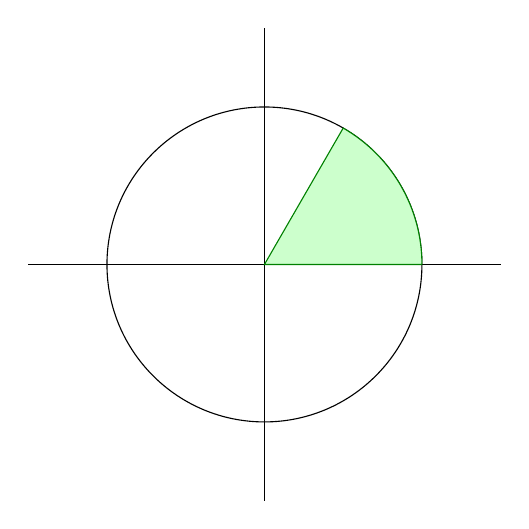
\begin{tikzpicture}
\draw (0,0) circle(2);
\draw (-3,0) -- (3,0);
\draw (0,-3) -- (0,3);

%Green Fill Arc
\filldraw[fill=green!20,draw=green!50!black] (0,0) -- (2,0) arc (0:60:2) -- cycle;
 \end{tikzpicture}
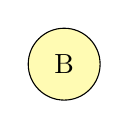
\begin{tikzpicture}
\node[draw, circle, fill=yellow!30, inner sep=2mm] (a) {B};
\end{tikzpicture}
\quad\quad

\begin{tikzpicture}
\shade (0,0) rectangle (2,1)
(3,0.5) circle (.5cm); 
\end{tikzpicture}

\quad\quad

cone\\\\

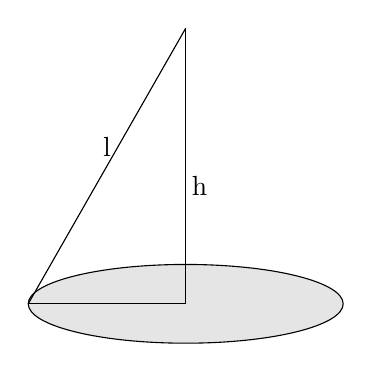
\begin{tikzpicture}
\filldraw[fill=gray!20](0,0) ellipse (2cm and 0.5cm);
%\draw (4,0) circle (2);
\draw (0,0) -- node[below] {\ \ \ h}(0,3.5);
\draw (0,0)  -- (-2,0);
\draw  (-2,0) --node[above] {l}(0,3.5);
\end{tikzpicture}\\\\
Circle Macro bluecircle Called \\\\\\
\begin{tikzpicture}
\bluecircle
\end{tikzpicture}


\begin{tikzpicture}
      \draw[->] (-3,0) -- (4.2,0) node[right] {$x$};
      \draw[->] (0,-3) -- (0,4.2) node[above] {$y$};
      \draw[scale=0.5,domain=-3:3,smooth,variable=\x,blue] plot ({\x},{\x*\x});
      \draw[scale=0.5,domain=-3:3,smooth,variable=\y,red]  plot ({\y*\y},{\y});
    \end{tikzpicture}





\end{document}


